\section{Experimental Protocol}
\subsection{Task Suite and Physical Verification}
The study includes controlled two-dimensional thermal design, a flagship mixed-cooling data-center layout task with supporting air-cooled configurations, and aerodynamic design. The source and closure models, fidelity levels, admissible designs, physical validation, and state-lifting contracts are frozen per scenario. A project schema check or small numerical gate is not evidence that the complete task suite is solved.

The first controlled pilot changes lid speed, heat-boundary location, and lid direction in a coupled Boussinesq cavity, using a version-pinned finite-volume residual and an implicit adjoint. It is a mechanism pilot for continuous and small discrete decisions. The broader controlled task includes varying heat-source and boundary configurations and admissible obstacles; generalization and all-high-fidelity training are separate requirements. Pilot success does not replace this task expansion. Its common analytic mechanical term is handled identically by strong baselines and reported separately from the fidelity-dependent thermal objective, so a separable known term cannot manufacture an apparent information gain. Manufactured-solution checks, conservation, boundary conditions, refinement, directional sensitivities, repeated-solve noise, and branch/initialization dependence are verified before interpreting learning results.

The principal data-center playground is the authored Shinaide mixed-cooling project, with its server inventory, cold plates and CDU. The registered equipment catalog and single-unit-outage requirement lead to a six-ACU research reference derived from this project; the authored four-unit geometry retains its source identity. The research task retains the cold plates and liquid routes while explicitly using the saved server airflows for fan-assisted operation. Figure~\ref{fig:shinaide} shows the six compiled architecture references. Its retained geometry, loads and equipment parameters carry explicit synthetic-input provenance. The coupled evaluation protocol requires an accepted liquid solution and heat-removal record, the corresponding residual room heat supplied to the air solver, and per-device closure $Q_{\rm IT}=Q_{\rm air}+Q_{\rm liquid}$. Air-side, liquid-side and shared-plant electricity are counted once. The initial steady benchmark prescribes cold-plate generation: the two subsystems share a fixed device heat budget, while controls change thermal margins and hydraulic and electrical costs. Thermal limits are attached separately to the air, solid and coolant quantities represented by the models. Pure-air engineering fixtures verify the compiler, boundary conditions and geometry before the full coupled task is accepted.

For the data-center scenario, equipment counts are fixed per task. The policy chooses containment, row direction/layout, compatible supply/return architecture, ACU shape/placement, and continuous supply temperatures, flows, aisle dimensions, and offsets. Mixed-cooling designs additionally expose liquid-side placement, routes and operating controls verified by the engineering compiler. The air-cooled v1 energy specification couples chilled-water reset, chiller efficiency, tower/pump energy and fan heat; both fidelities use the same accounting module. Total design-condition PUE is the primary objective. Air-cooled configurations retain exhaust temperature or thermal margin as a lower-weight secondary objective and server inlet/exhaust constraints; the mixed-cooling specification adds the corresponding solid and coolant limits. Geometry, airflow closure, leakage, coil capacity, dew-point checks, and N+1 behavior belong to the declared task contract. Numerical limits, equipment assumptions and their evidence status are pinned in the task specification before training; synthetic values are distinguished from equipment calibration.

The high-fidelity pipeline is an actual candidate \texttt{.cfdproj} through geometry/mesh export, physical solve, and face-based post-processing. A small headless export witness establishes its own interface only; room generation, containment, supply/return routing, boundary fingerprints, and the selected architecture menu require separate tests. L0 is a differentiable zonal model. L1 is coarse CFD or a field-producing calibrated surrogate; only L1 can supply the field required for target residual evaluation. Complete and energy-only residual interfaces are reported separately.

The aerodynamic protocol uses 16 reference-preserving upper/lower CST perturbations and DAFoam RANS~\cite{he2020dafoam}. Drag is minimized under lift and geometry constraints. Requirements vary Reynolds number, reference geometry and operating conditions; angle of attack is supplied by the task. A differentiable panel model with a declared drag closure and coarse/fine RANS provide distinct information interfaces. Surface mapping, total shape derivatives and grid quality require verification before policy training. The separately recorded native lift and official drag/angle gates are interface history, not results on this new benchmark. A data-center adjoint interface remains a separate study requirement.

Training, calibration, validation, final test, and out-of-distribution sets are separated by physical task and geometry identity. Paraphrases of a task stay in one split. Heuristic SFT teaches the format and legal proposal construction; optimizer-generated high-fidelity reference designs are not silently imported into the common initialization. They are permitted in a separately costed distillation baseline. Every structured baseline receives equivalent requirements and constraints.



\begin{figure*}[t]
\centering
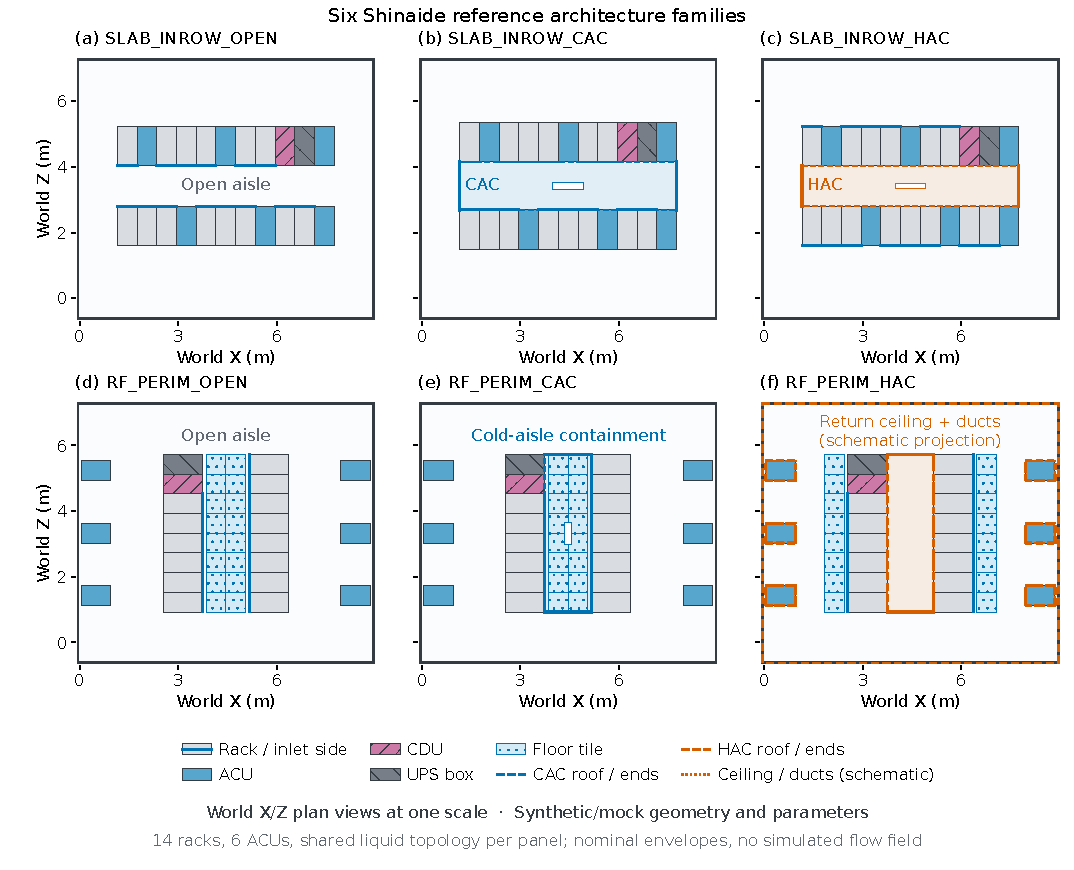
\includegraphics[width=\textwidth]{figures/shinaide_six_family_plans.pdf}
\caption{Six compiled Shinaide architecture references: slab-floor in-row cooling (top) and raised-floor perimeter cooling (bottom), each with open aisles, cold-aisle containment or hot-aisle containment. All panels share the same room coordinates and scale. Equipment envelopes, rack inlet sides, containment sheets and floor tiles come from the saved projects; ceiling returns and vertical ducts are schematic projections. Each reference retains 14 racks, 56 server models, six ACUs and one CDU, with explicit synthetic/mock provenance. These are reference designs, not optimized outcomes or flow fields.}
\label{fig:shinaide}
\end{figure*}

\subsection{E1--E8 Study Matrix}
\textbf{E1: information effects.} A preregistered fractional factorial design studies component controls, residual features, sensitivities, target correction, acquisition, and conditional discrete enumeration. Every cell must correspond to an available interface. The alias matrix and estimable contrasts are recorded so interactions are not inferred from confounded or undefined cells. Scalar-only, pure-HF, pure-L0, and multi-fidelity settings are retained as declared comparison blocks. All policy methods use the numerical head; a digital-token interface comparison is separately isolated.

\textbf{E2: cost--quality frontier.} Sweep target budgets from zero to the all-high-fidelity reference. Zero-target training belongs to the explicit proxy regime, not the corrected estimator. Plot quality and constraint satisfaction against complete CPU/GPU cost and wall time. Controlled tasks supply a tractable all-high-fidelity training reference; it is not assumed to be the global optimum.

\textbf{E3: target information interfaces.} Compare black-box target feedback, surrogate derivatives, residual-only feedback, residual-plus-adjoint output correction, and a validated target adjoint. Complete interface variants are studied where available, with their measured lifting, closure, meshing, and backward costs. The black-box data-center study does not establish its unimplemented adjoint variant.

\textbf{E4: strong method comparisons.} Principal baselines are MFPG-PPO including budget management, faithful nested MFPG/REINFORCE or RLOO, and prediction-powered correction with nonphysical uncertainty~\cite{liu2025mfpg,liu2026mfpgppo,angelopoulos2024ppipp}. HPO, learned differentiable controls, ABC/DAE, and adaptive-bias ABC-Align provide distinct gradient/critic or semi-supervised comparisons~\cite{alvo2026hpo,grathwohl2018relax,pan2026abc,frankel2026abcalign}. Other target-feedback uses include pooling, low-fidelity pretraining followed by target fine-tuning, L0 screening with target-verified self-training, optimizer-to-SFT distillation, on-policy discrepancy-model refresh, and uncertainty penalties. Adaptations preserve each baseline's defining mechanism and receive the same tuning and total evaluation budget.

\textbf{E5: policy and amortization.} Compare a heuristic designer; CMA-ES, multi-fidelity BO, and adjoint descent on the same design parameterization; and an equivalently informed structured neural policy using the same estimator. Report learning/setup cost, deployment cost, task quality, and break-even workload. The need for a language backbone is evaluated across changing and compositional requirements, not inferred from a single task.

\textbf{E6: inference-time agents.} Use the original Qwen policy with the same harness, a named frontier model with a pinned version and equivalent tool/cost budget, Phythesis/SGA-style refinement, and language-generated structure followed by per-task L0 gradient refinement and target validation~\cite{li2025phythesis,ma2024sga}. Common-prompt, common-tools, and common-validation protocols isolate the net benefit of post-training.

\textbf{E7: generalization.} Hold out requirements, geometries, room/equipment scales, equipment placement, architecture combinations, and wording. The 4B and 27B configurations are distinct required study arms, with model hashes and measured numerical-head/adapter memory. Larger-model execution remains under the existing single-GPU authorization; footprint verification is a prerequisite, not evidence of a learning result. Cross-scenario transfer and a joint-scenario policy are reported separately from within-scenario generalization.

\textbf{E8: verification fidelity.} Audit representative final candidates with refined meshes and, where required by flow behavior, transient or repeated-initialization checks. Report changes in feasibility and objective ranking, including computational failures and target-model sensitivity. Optimization of the training evaluator is distinguished from reliability under this additional physical check.

\subsection{Estimator Audit, Regimes, and Ablations}
At preregistered frozen checkpoints, repeated independent batches compare mean error, covariance trace, gradient alignment, and MSE at matched total cost relative to a high-accuracy reference gradient with its own quantified numerical and sampling uncertainty. A finite Monte Carlo reference is not labeled an exact gradient. This is the main mechanism evidence for target consistency and cost allocation. Predictable and HT peer baselines, uniform nesting, multiple controls, and randomized acquisition are tested separately. When RLOO is used, the independent replication unit is a complete prompt group and the audit retains its covariance structure.

The corrected and trusted-proxy regimes are explicitly labeled. A controlled discrepancy concentrated in the policy's frequently visited region probes proxy exploitation. Residual-based acquisition, residual-based substitution, and objective/adjoint correction are separate interventions. A sign-flipped cheap reward is only a sanity check: an adaptive control coefficient can compensate for its sign without demonstrating resistance to realistic policy-distribution shift.

Ablations include scalar versus component controls; residual gates versus residual features; exact versus approximate adjoints; exact versus approximate path derivatives; LAX versus matched auxiliary-vector use; fixed versus calibrated coefficients; uniform, fixed-budget, and randomized objective-aware acquisition; enumeration/RELAX versus score estimation; and numerical heads versus numerical tokens. Direct-path, adaptive-mixing, residual-as-reward, and RLVP-style reward-shape variants isolate the associated ideas~\cite{nel2025grade,son2023gippo,yuan2025pirf,cai2026rlvp}. They are named adaptations or ablations, not purported reproductions on the original output domains.

\subsection{Statistics, Quality, and Complete Costs}
Confirmatory controlled-scene comparisons use at least ten independent training seeds and data-center comparisons at least five. The aerodynamic protocol targets at least five and freezes its final count before training. Pilot runs may be smaller but cannot substitute for these comparisons. Common random numbers couple eligible task evaluations; the estimator's independent replications remain distinct. IQM, paired effect estimates, and hierarchical bootstrap intervals preserve task and seed structure. At most three primary hypotheses are preregistered and receive Holm correction; other analyses are labeled exploratory. These counts are protocol minima, not universal power guarantees.

For the launched controlled study, the fixed-budget analysis uses the latest scheduled checkpoint available at each charged budget, on the common support of all method--seed runs. It does not choose the best observed checkpoint or interpolate unobserved quality. Failed outcomes retain their registered reward and incurred costs. The prepared descriptive intervals resample entire paired training-seed blocks, keeping the two validation tasks fixed; these pointwise intervals do not establish generalization to a task population. This analysis specification was recorded after training launch and before aggregate outcome access, so it is not presented as a pretrial statistical preregistration. Confirmatory tests and any multiplicity correction require a separately frozen hypothesis protocol.

Final task quality uses the same target evaluator. Report feasible completion, constraint violations, hidden-specification satisfaction, and objective quality among feasible designs separately. Server temperatures use declared inlet/exhaust face statistics, rather than unqualified sparse probes. Cooling power, design-condition PUE contributions, RCI/RTI/SHI/RHI, and plant temperatures have pinned definitions. Optimizer search supplies a \emph{best-found, target-verified} reference unless a true bound is certified; signed improvements beyond it are not clipped or recast as impossible.

Full target evaluation is required for displayed accepted design examples and the declared confirmatory test subset. A secondary large-population mean may use a prediction-powered or inclusion-weighted evaluation with randomized target labels~\cite{angelopoulos2024ppipp,zrnic2024active}. That estimate does not imply that every design was physically checked. Applying it to IQM, quantiles, or maxima requires an appropriate functional estimator and its uncertainty, not reuse of a mean formula.

The ledger records generation tokens/time, optimization/backpropagation, calibration, surrogate data/training, compile/export, L0, L1, residuals, adjoints, mesh, solve, post-processing, queueing, retries, and failures. Shared costs are charged once; GPU/CPU conversion is fixed in advance and tested for sensitivity. Cold/warm caches are declared with complete design and boundary fingerprints. Failure cost is recorded on each attempt under the common retry policy. Retrospective success-rate inflation is not added to the same attempt costs.

\subsection{Execution and Completion Evidence}
Every run has an immutable case-local dated logger with code, dependency/evaluator, model, case/project, task-split, seed, configuration, acquisition-probability, cost, checkpoint, and terminal-status identity. A hard candidate is compiled from the recorded agent output, and the evaluated design must match its saved project and solver inputs. Schema-valid artifacts, correct estimator unit tests, physical evaluator gates, short model runs, and confirmatory research experiments are separate evidence levels.

The complete implementation work is tracked as W0--W12: platform repair/security/headless export, task specification, task/prompt generation, DSL/project compiler, energy model, zonal model, target CFD/calibration, metrics/reward, harness, cost ledger, analysis, baselines/reference search, and SFT/RL integration. The residual and adjoint interfaces are additional tracked dependencies. Their acceptance conditions and E1--E8 evidence are maintained in the repository's requirements-to-evidence audit; the study is not complete when only its first physics or software gate passes.

Weak or inconsistent learning first triggers checks of implementation, gradients, physical validity, data/splits, metrics, and budget/tuning fairness. Corrected evidence then determines the supported strengths and operating scope. Reports preserve counterexamples and original failed runs while removing falsified claims. Results enter this manuscript only after independent source-level verification.
